% Author: Taejin Hwang
% Email: taejin@berkeley.edu

\qns{Interpolation Stability}

\meta {
  The following paragraphs below explain the motivation behind interpolation, and what the goal of interpolation is. 
  We then use the only technique of interpolation that we know, which is Lagrange Interpolation, but show its issues to motivate a better form of interpolation through the Fourier Transform.
}

In the controls module of the course, we saw the notion of taking a continuous function $x(t),$ and taking \textbf{samples} at equally spaced intervals $T$ to get samples $x(nT)$ for integers $n = 0, 1, \ldots, N.$ 
Having a discretized version of a signal gives us a way in which we can store the information that a continuous time signal contains into a compact digital form. 
This form is desirable because computers are fundamentally discrete and can only process data that is stored digitally.

\meta {
  Example of signal processing shown below: Sampling audio, using a low pass to remove the noise, and then retransmitting it through a speaker. To motivate the material, you may want to draw out the signals $x(t), x[n], y[n],$ and $y(t)$ so that students can see what each step is doing. If students ask about digital low-pass filters, tell them to not worry, and that it's implemented similar to an analog low-pass seen in Module 1 with circuits.
}

Here's an example of a digital signal processing system where we take a continuous time signal, sample it every $T$ seconds, apply a low-pass filter, and then interpolate it back into a continuous time signal to transmit.
\tikzstyle{int}=[draw, fill=blue!20, minimum size=2em]
\tikzstyle{init} = [pin edge={to-,thin,black}]
\begin{center}
  \begin{tikzpicture}[node distance=2.5cm,auto,>=latex']
    \node [int, pin={[init]below:$T$}, align=left] (a) {Sampling};
    \node (b) [left of=a,node distance=2cm, coordinate] {a};
    \node [int] (c) [right of=a, pin={[init]below:CPU}, node distance = 5cm, align=center] {Low-Pass \\ Filter};
    \node [int] (d) [right of=c, node distance = 4cm, align=left, pin={[init]below:Interpolation}] {Transmitter};
    \node [coordinate] (end) [right of=d, node distance=2cm]{};
    \path[->] (b) edge node {$x(t)$} (a);
    \path[->] (a) edge node {$x[n] = x(nT)$} (c);
    \draw[->] (c) edge node {$y[n]$} (d);
    \path[->] (d) edge node {$y(t)$} (end);
  \end{tikzpicture}
\end{center}
We can do all of the signal processing digitally on a computer, but if we wanted to transmit this signal back into the real world, we want a way to now recover a continuous time signal from a discrete signal. The process of doing such is called \textbf{interpolation} and in this question we will take a closer look into the strengths and weaknesses of \textbf{Lagrange Interpolation.}

For the purposes of this question, suppose that we are taking samples every $T = \SI{1}{\second}$  from the following continuous time signal.

\begin{center}
  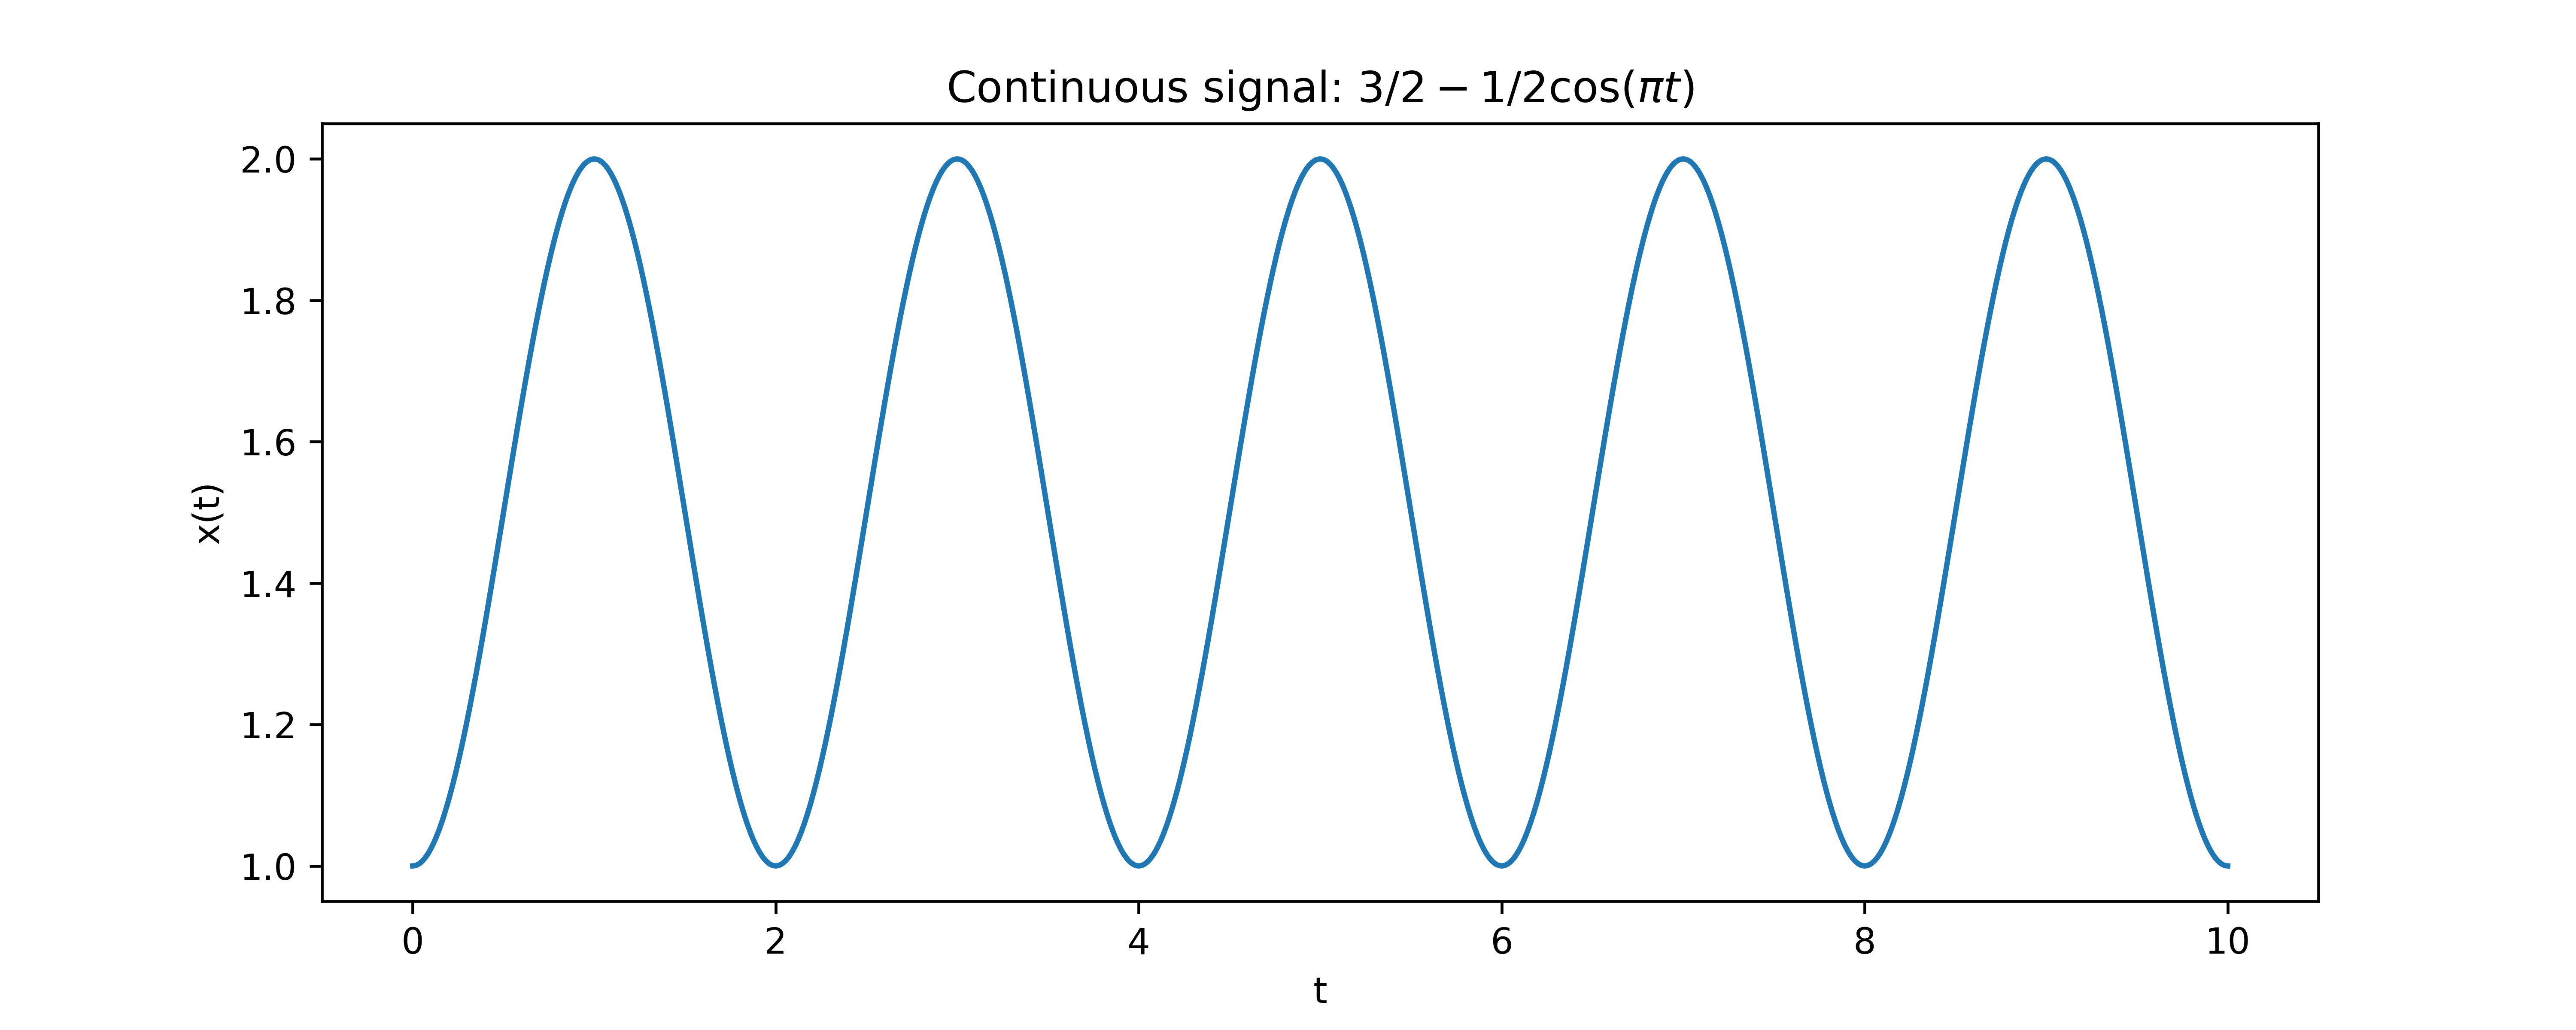
\includegraphics[width=6in]{\bank/interpolation/figures/ct_signal}
\end{center}

\newpage

\begin{enumerate}
  \qitem Let's start by taking two samples; one at $T = 0$ and another at $T = 1.$ 
  What is the interpolated Lagrange Polynomial for these two points?

  \ws {
    \begin{center}
      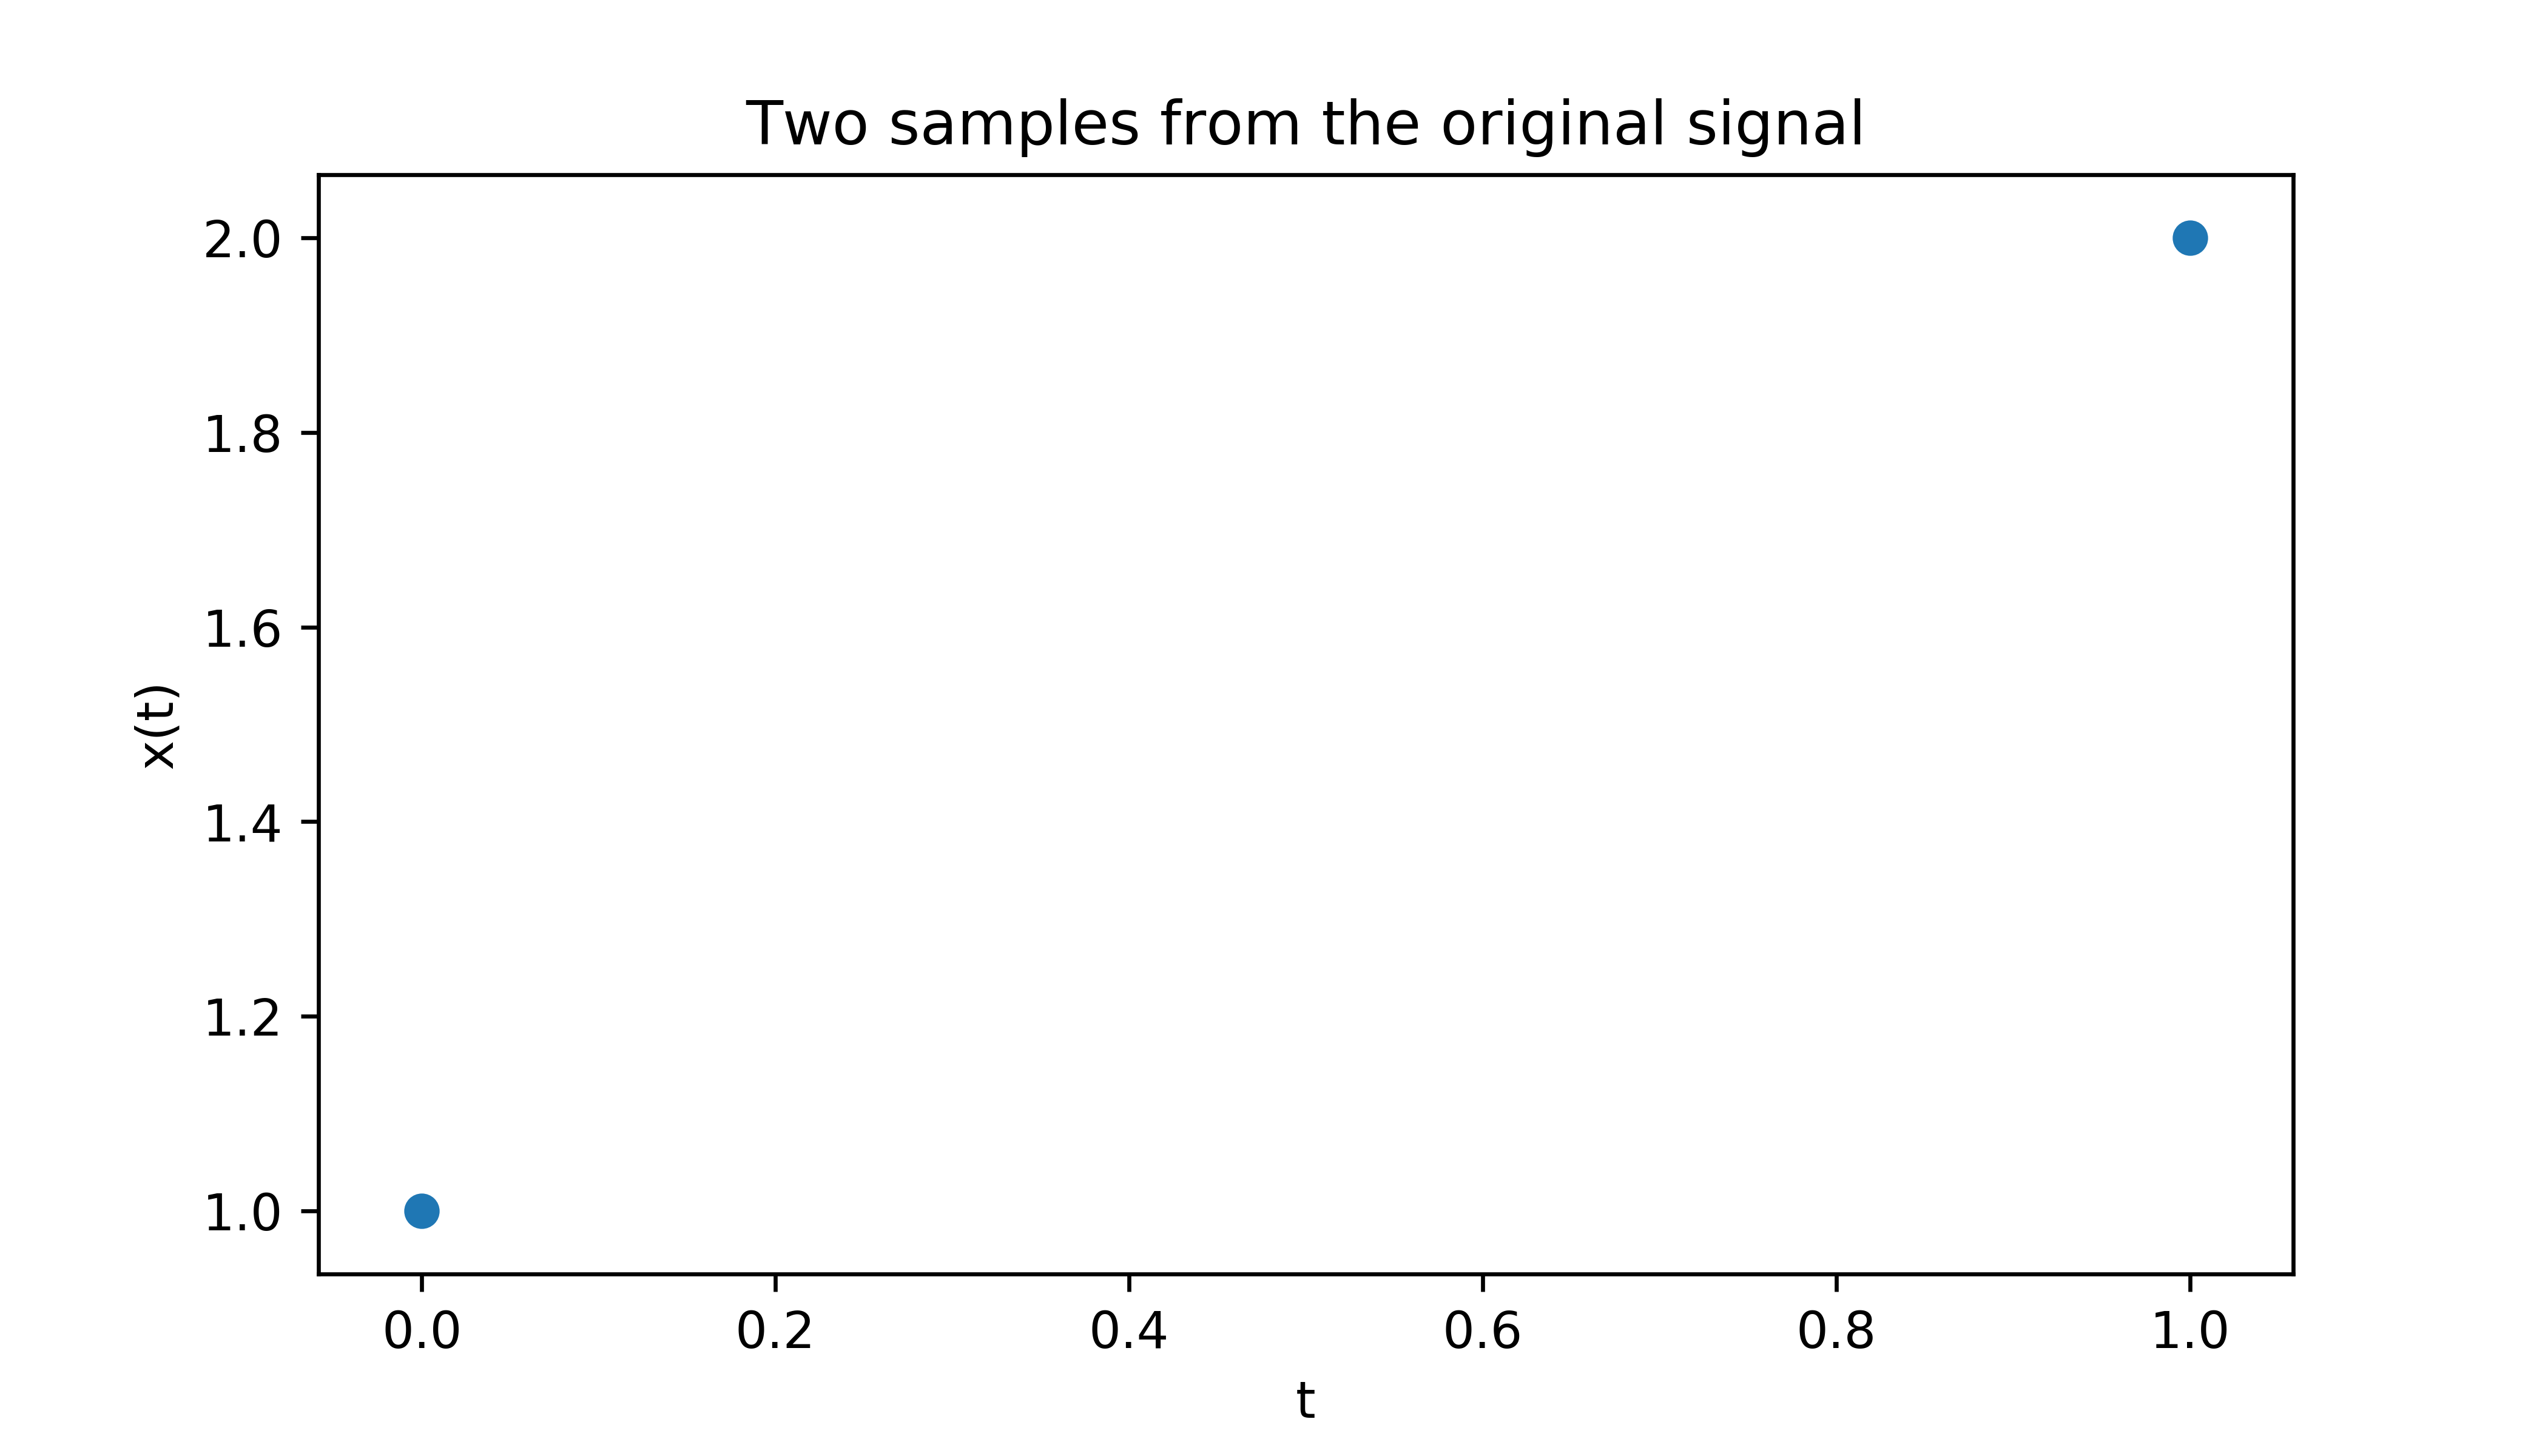
\includegraphics[width=5in]{\bank/interpolation/figures/two_pt_samples}
    \end{center}
  }

  \sol {
    Remember that for Lagrange Interpolation, we take $n$ sample points and interpolate a degree $n - 1$ polynomial. 
    In this specific case, we are given two points, so we want a polynomial of degree one, or a line. 
    Since the Lagrange polynomial must pass through all of the points, it should come naturally that the Lagrange Polynomial is the line $x(t) = t + 1.$ 
    \begin{center}
      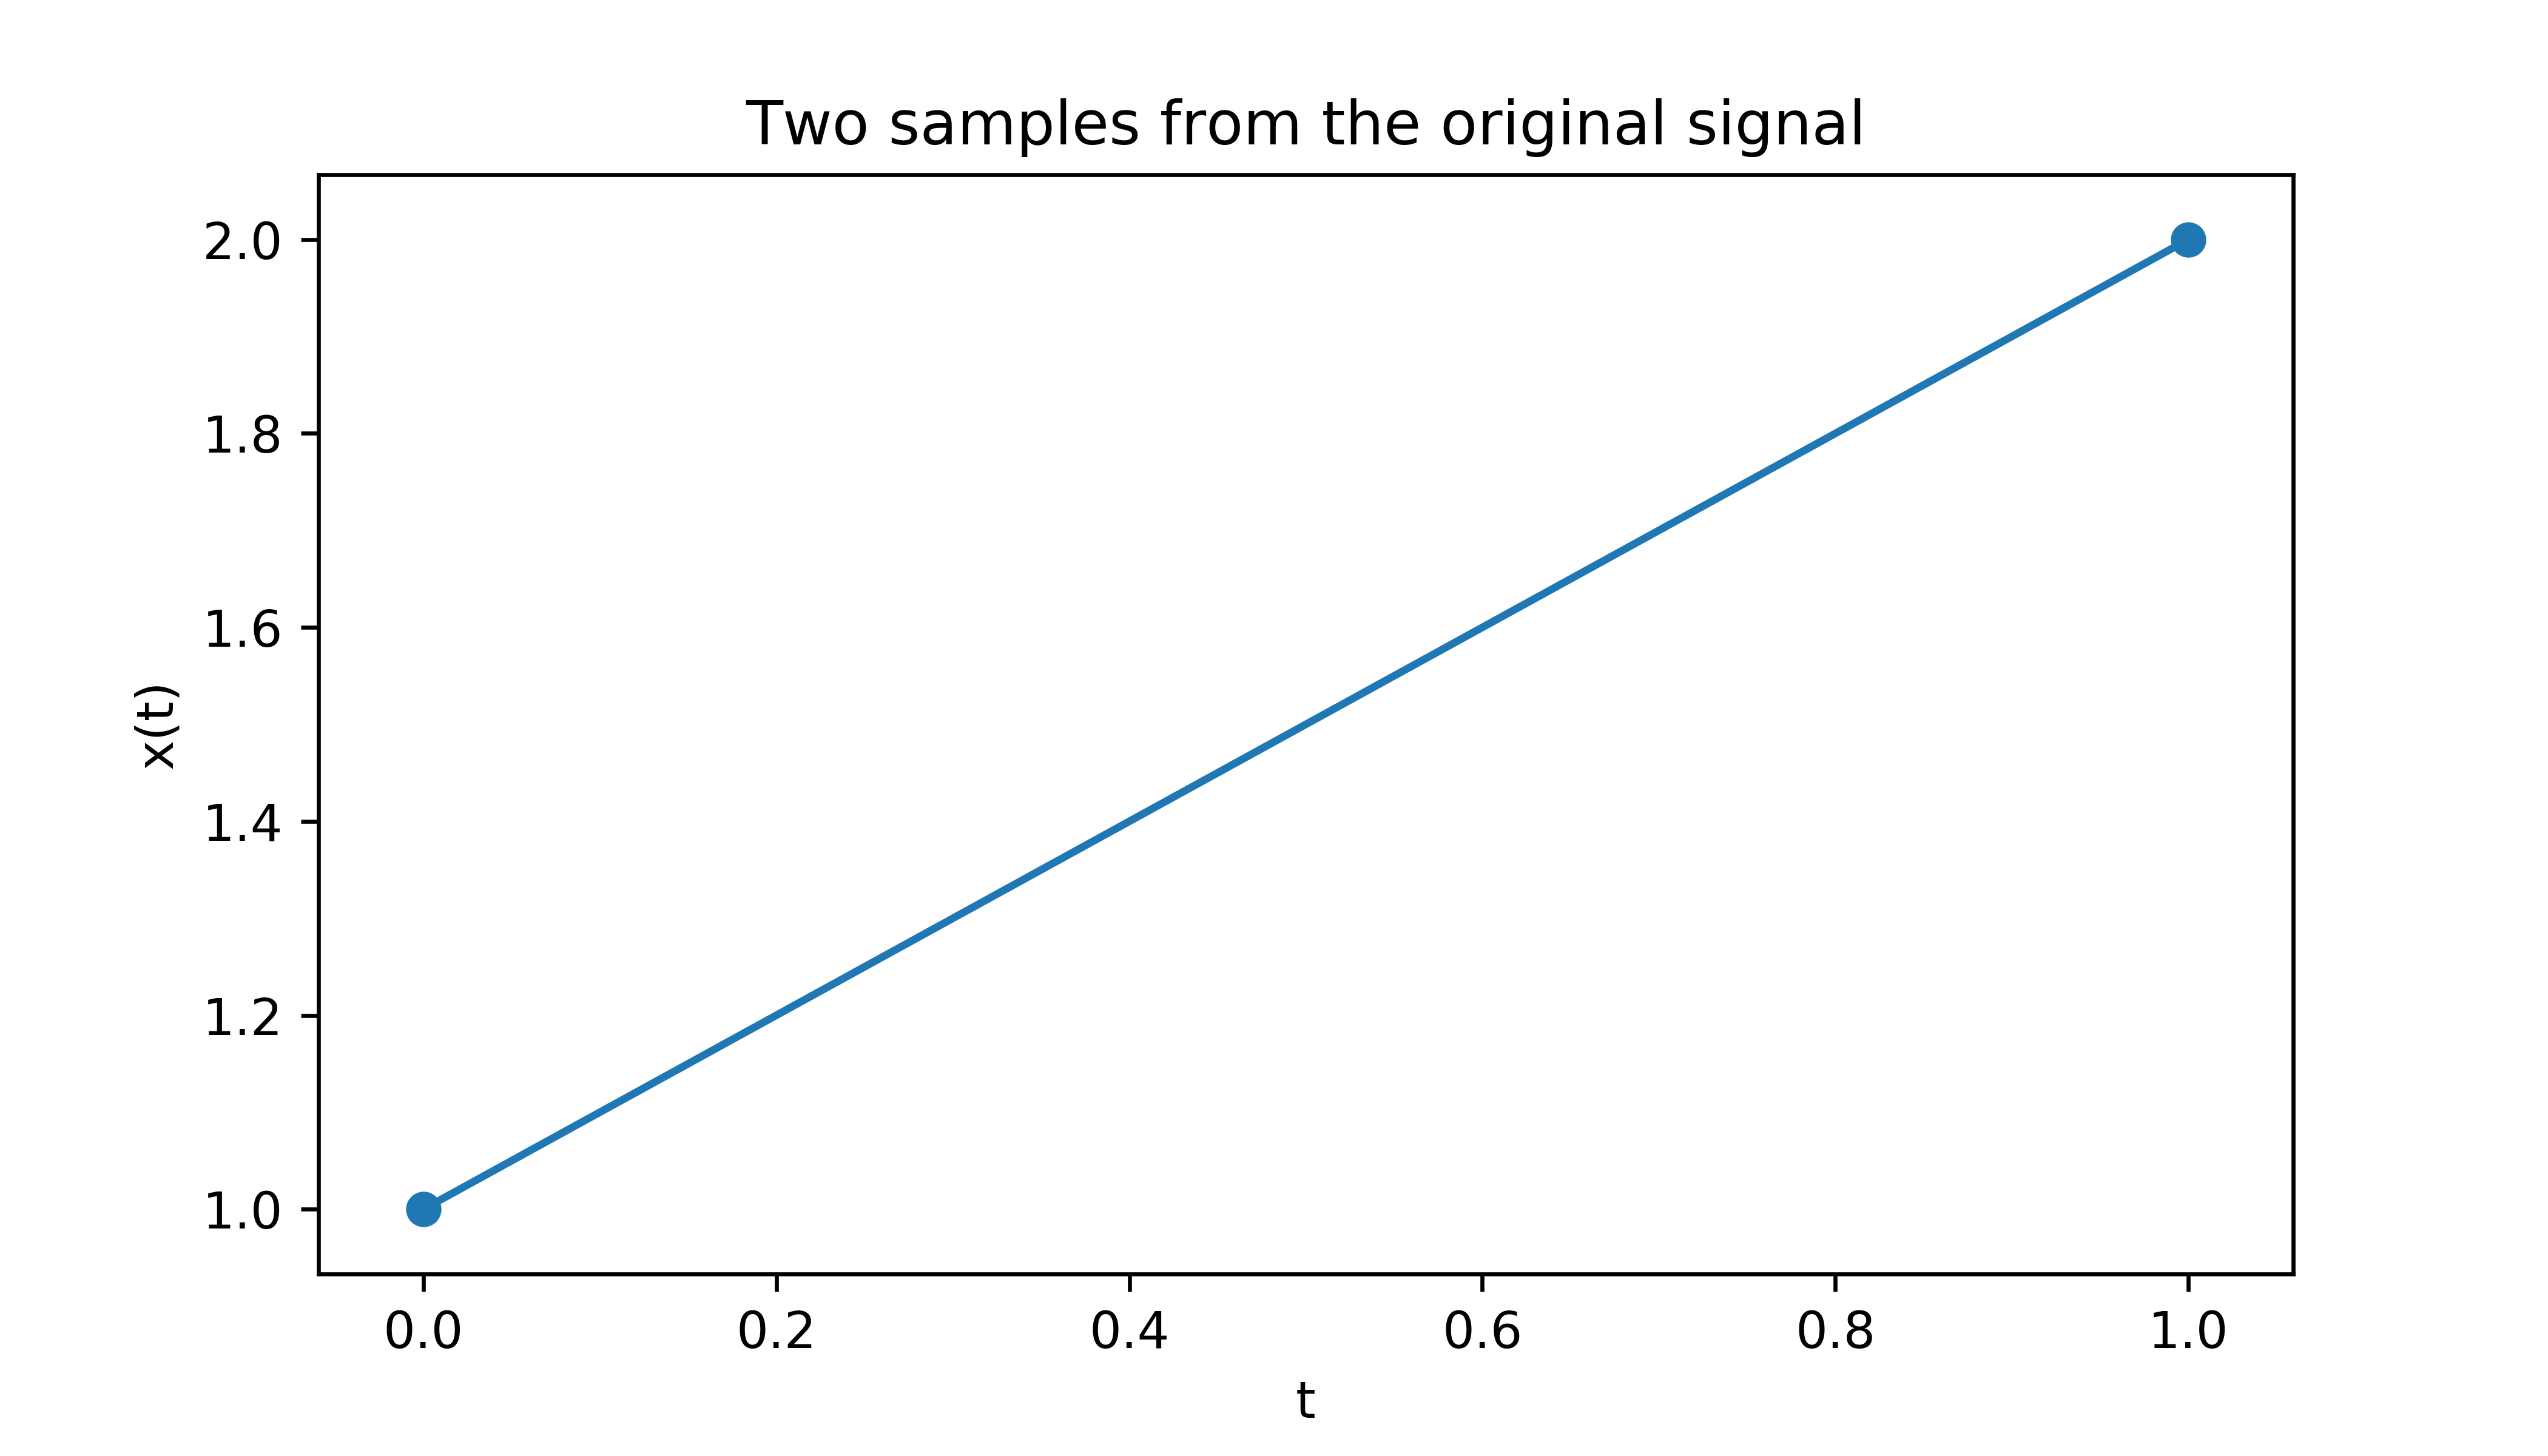
\includegraphics[width=5in]{\bank/interpolation/figures/two_pt_lagrange}
    \end{center}
  }

  \qitem Now let's take three samples for $T = 0, 1, 2.$ According to the figure below, what is the interpolated Lagrange Polynomial for these three points?

  \ws {
    \begin{center}
      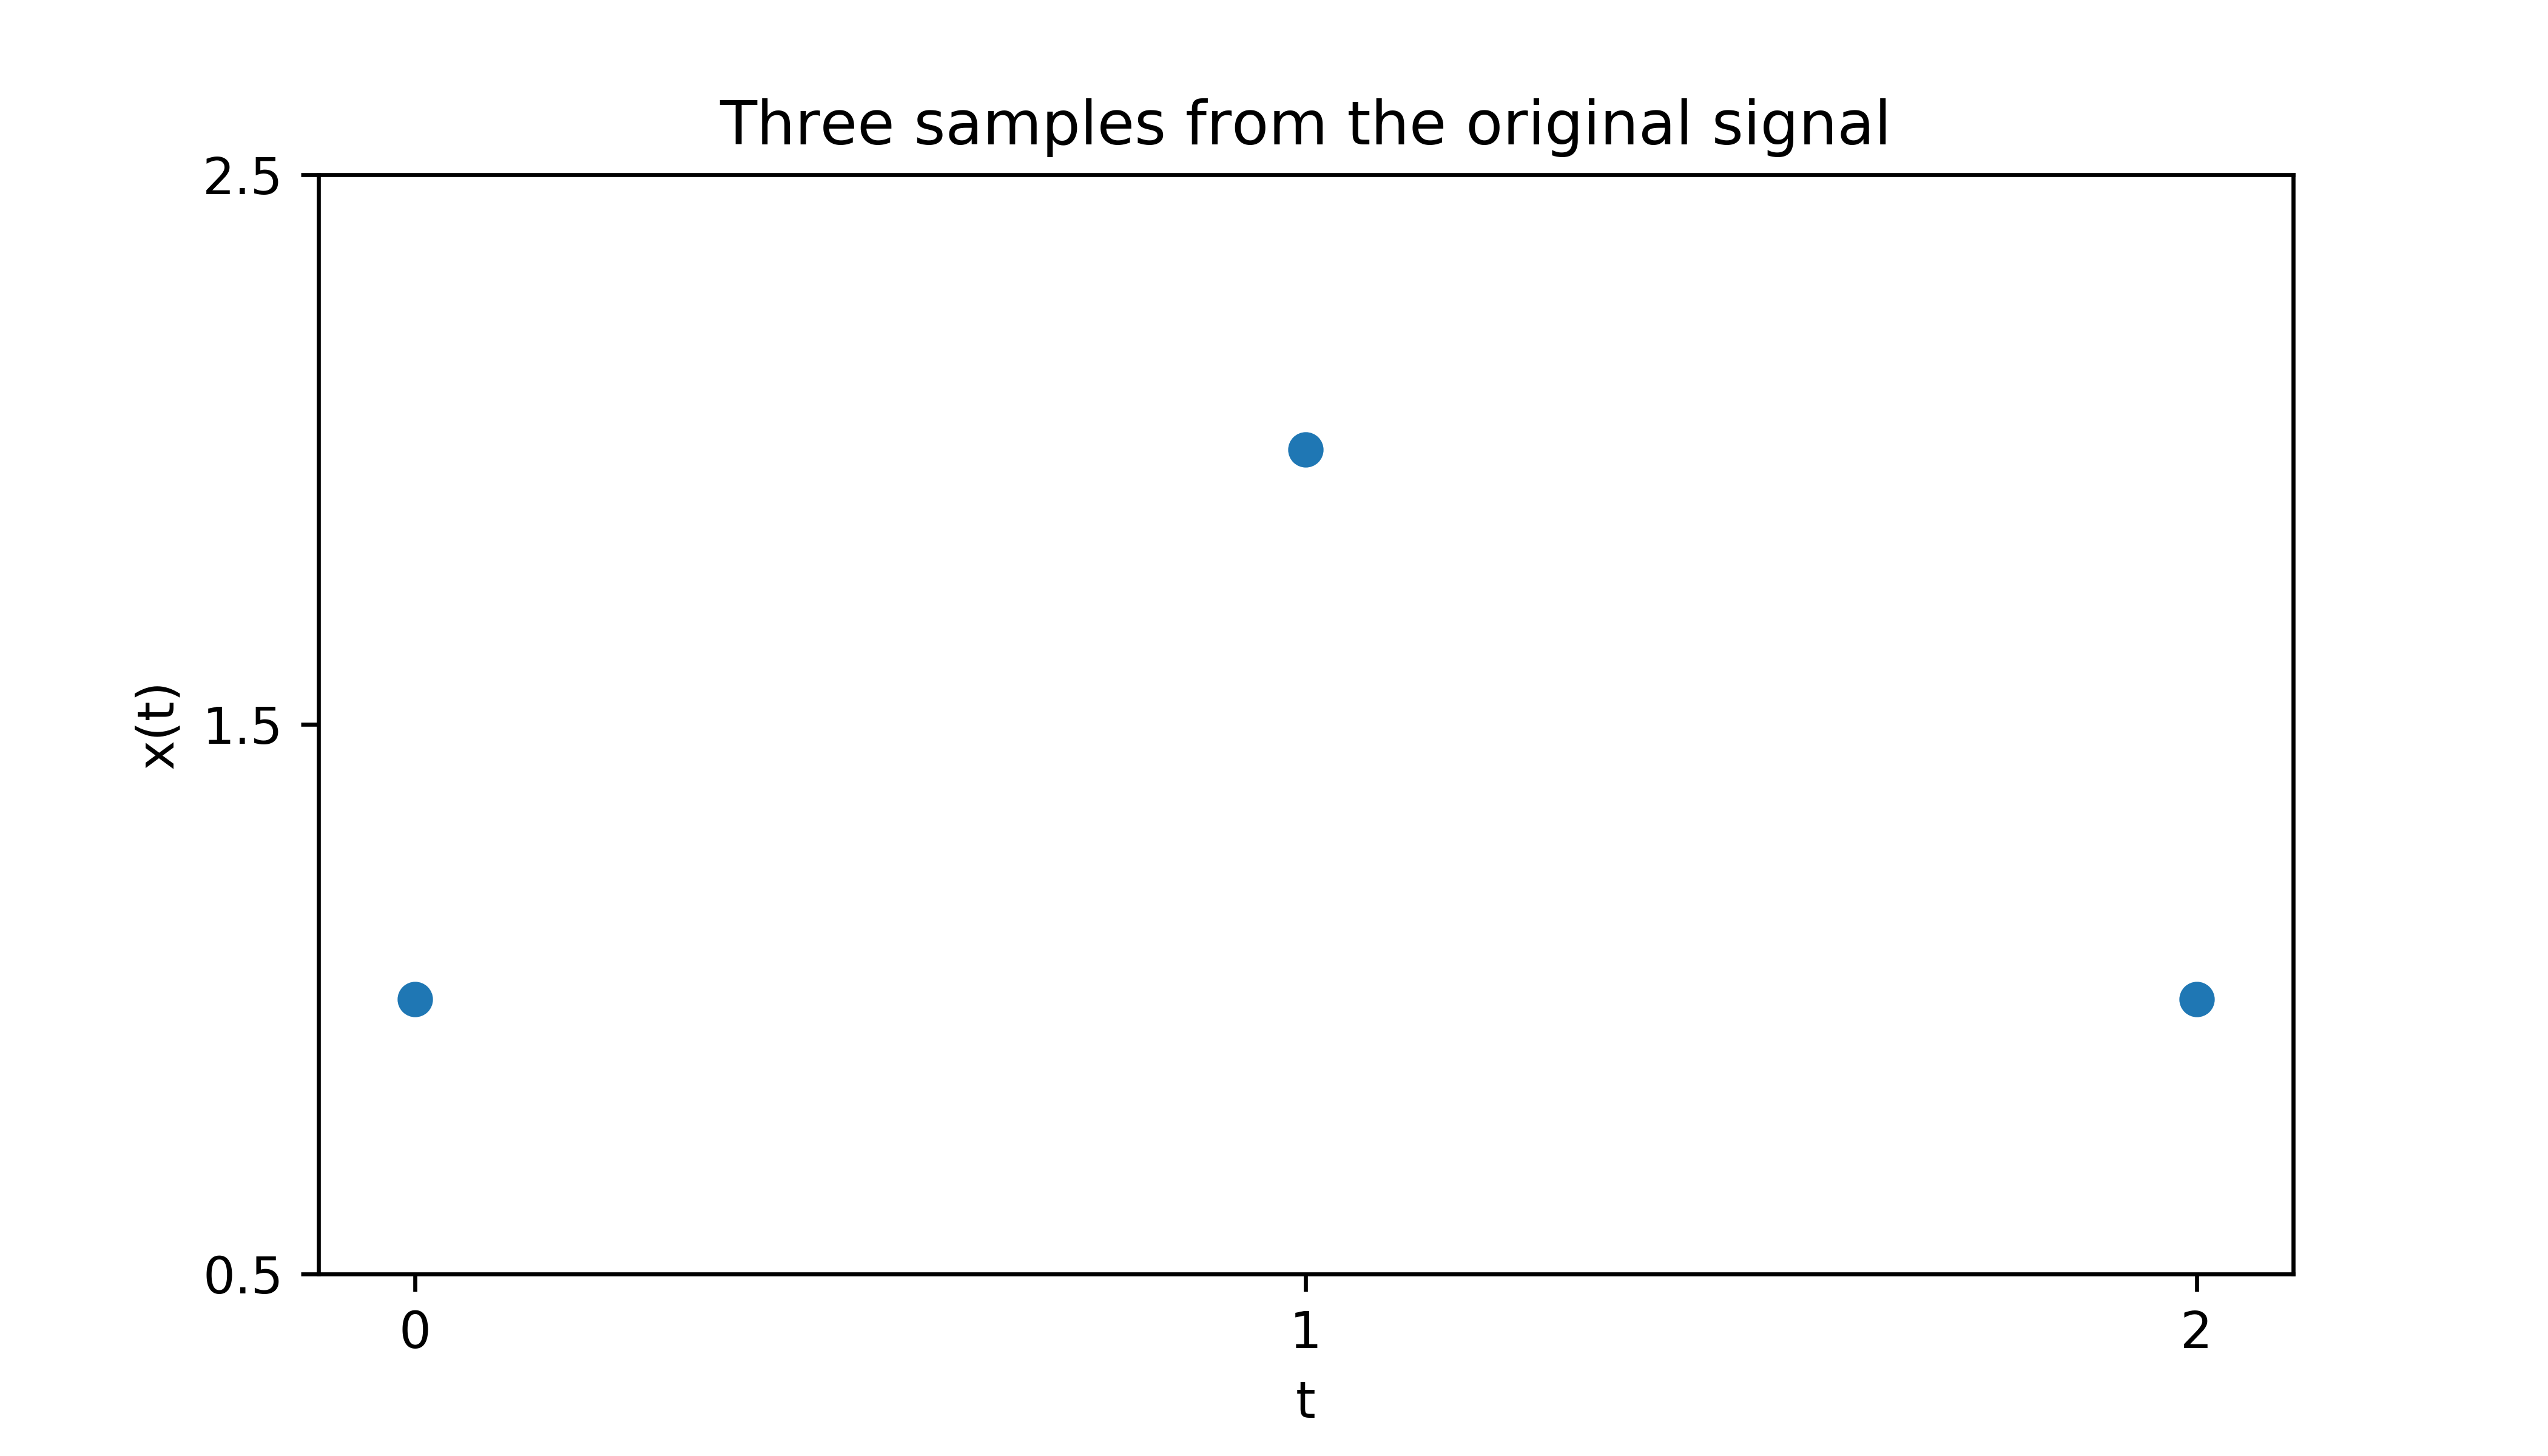
\includegraphics[width=5in]{\bank/interpolation/figures/three_pt_samples}
    \end{center}
  }

  \sol {
    We can resort to the Lagrange Polynomial formula and arrive at:
    $$x(t) = \frac{(t - 1)(t - 2)}{(-1)(-2)} + \frac{(t)(t - 2)}{(1)(-1)} + \frac{(t)(t - 1)}{(2)(1)} = -t^2 + 2t + 1.$$ 
    \begin{center}
      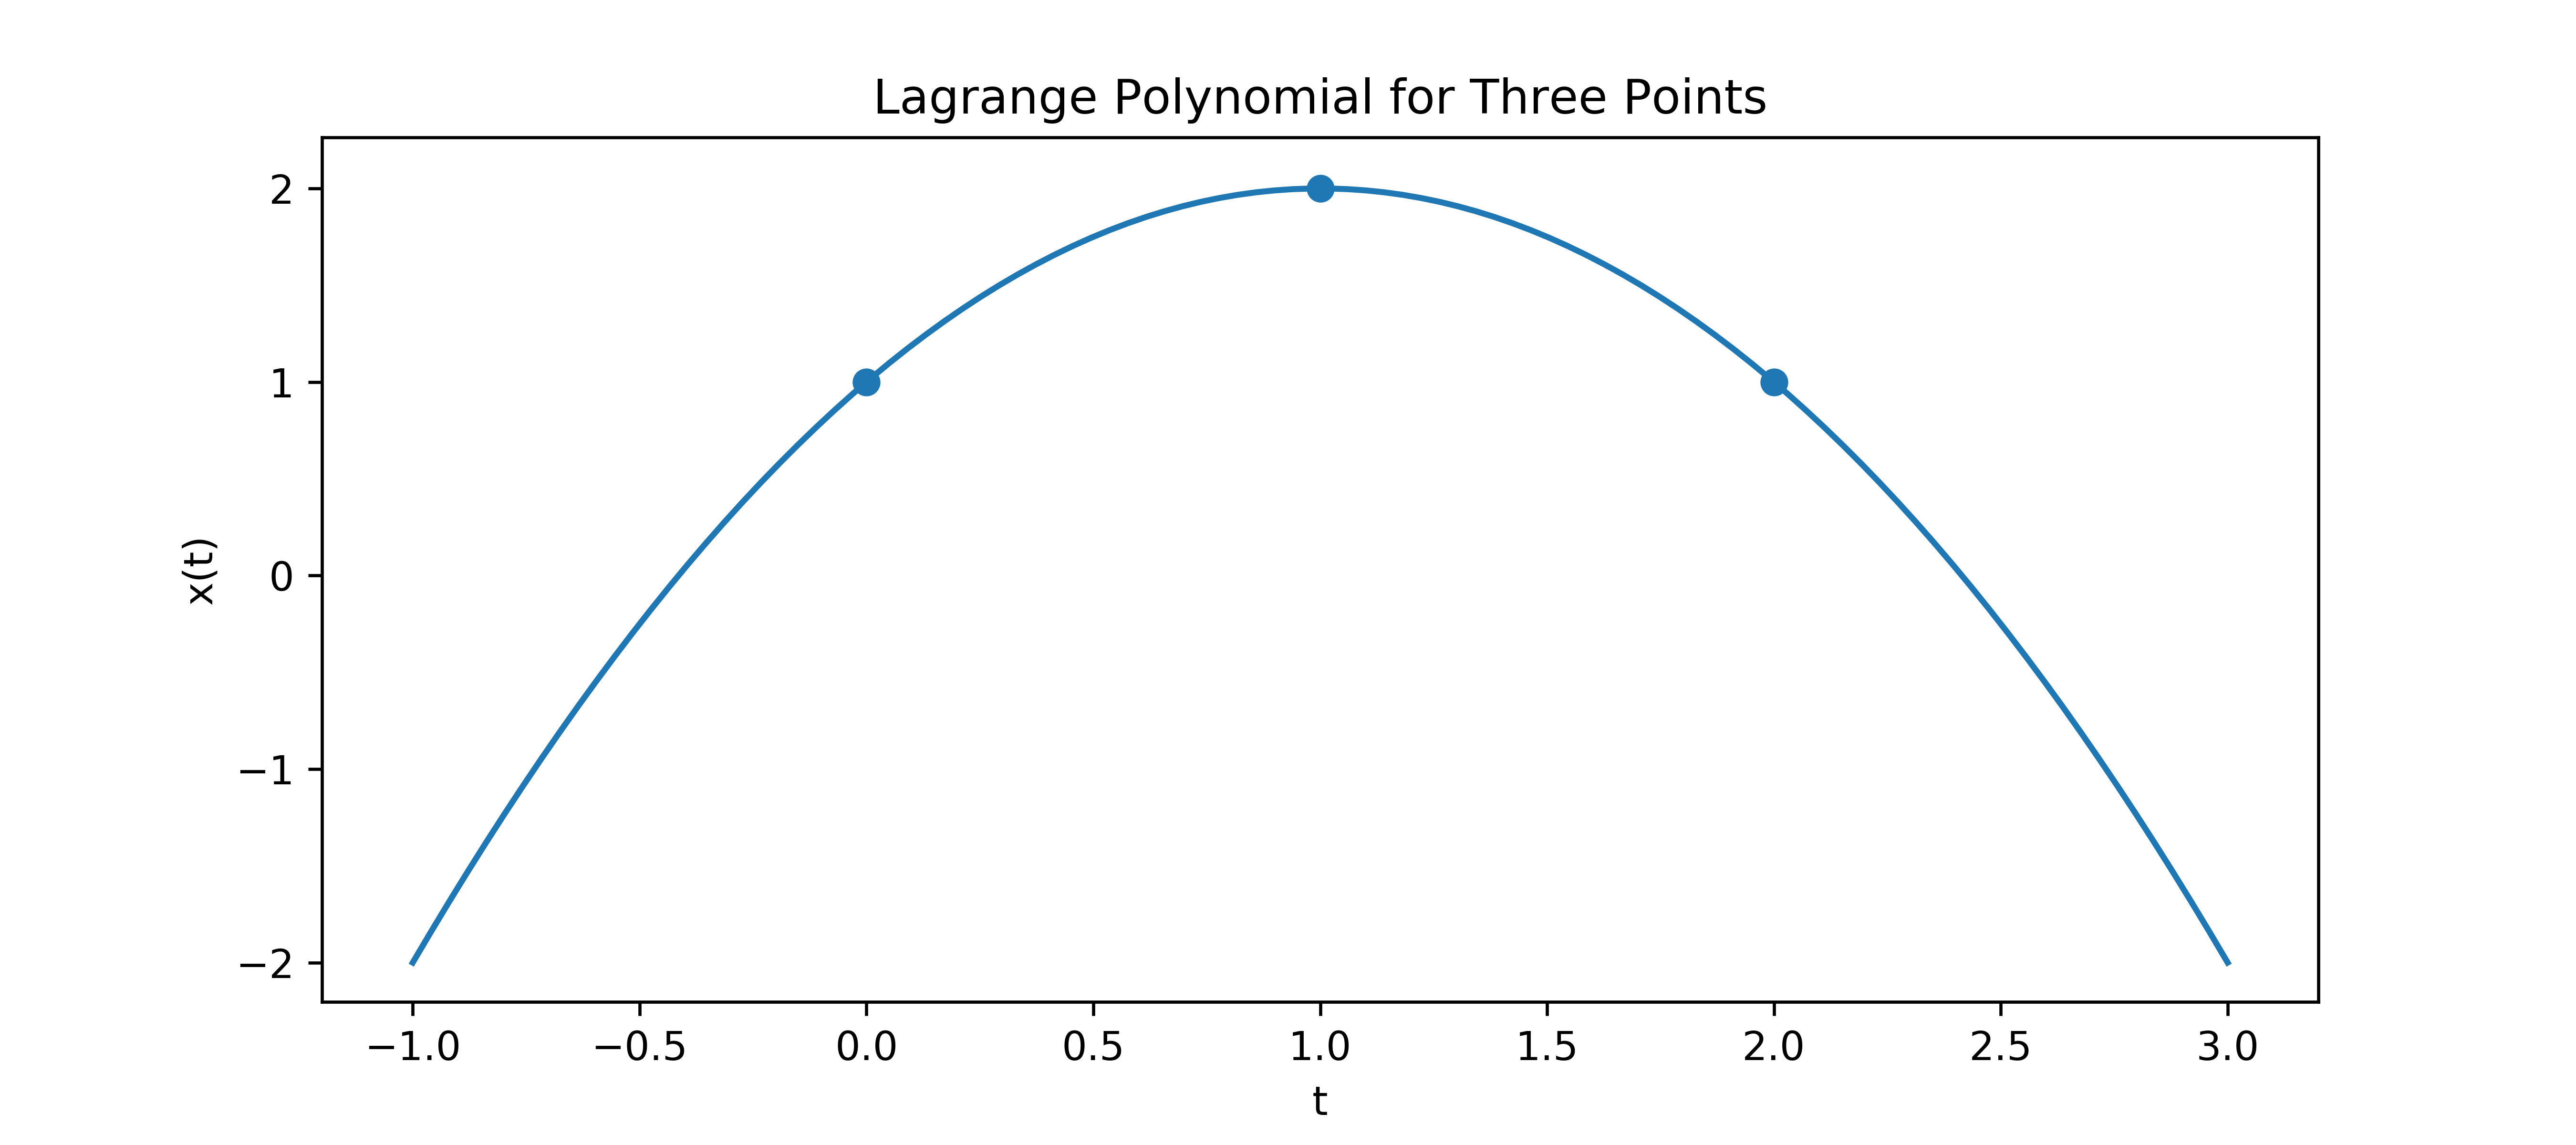
\includegraphics[width=6in]{\bank/interpolation/figures/three_pt_lagrange}
    \end{center}
    Or we can note that this polynomial passes through the y-coordinate $1$ at $T = 0$ and $T = 2.$
    We can take the polynomial with roots at $0$ and $2$ pointing downard, or $x(t) = -(t)(t - 2)$ and shift it upward by $1$ to get $x(t) = -t^2 + 2t + 1.$
  }

  \newpage
  
  \qitem Now let's add another sample, so that we have four samples total. What is the interpolated Lagrange Polynomial for these points? Also what are the evaluations of the polynomial at points outside the sampled range, for $t = -1$ and $t = 3?$ 


  \ws {
    \begin{center}
      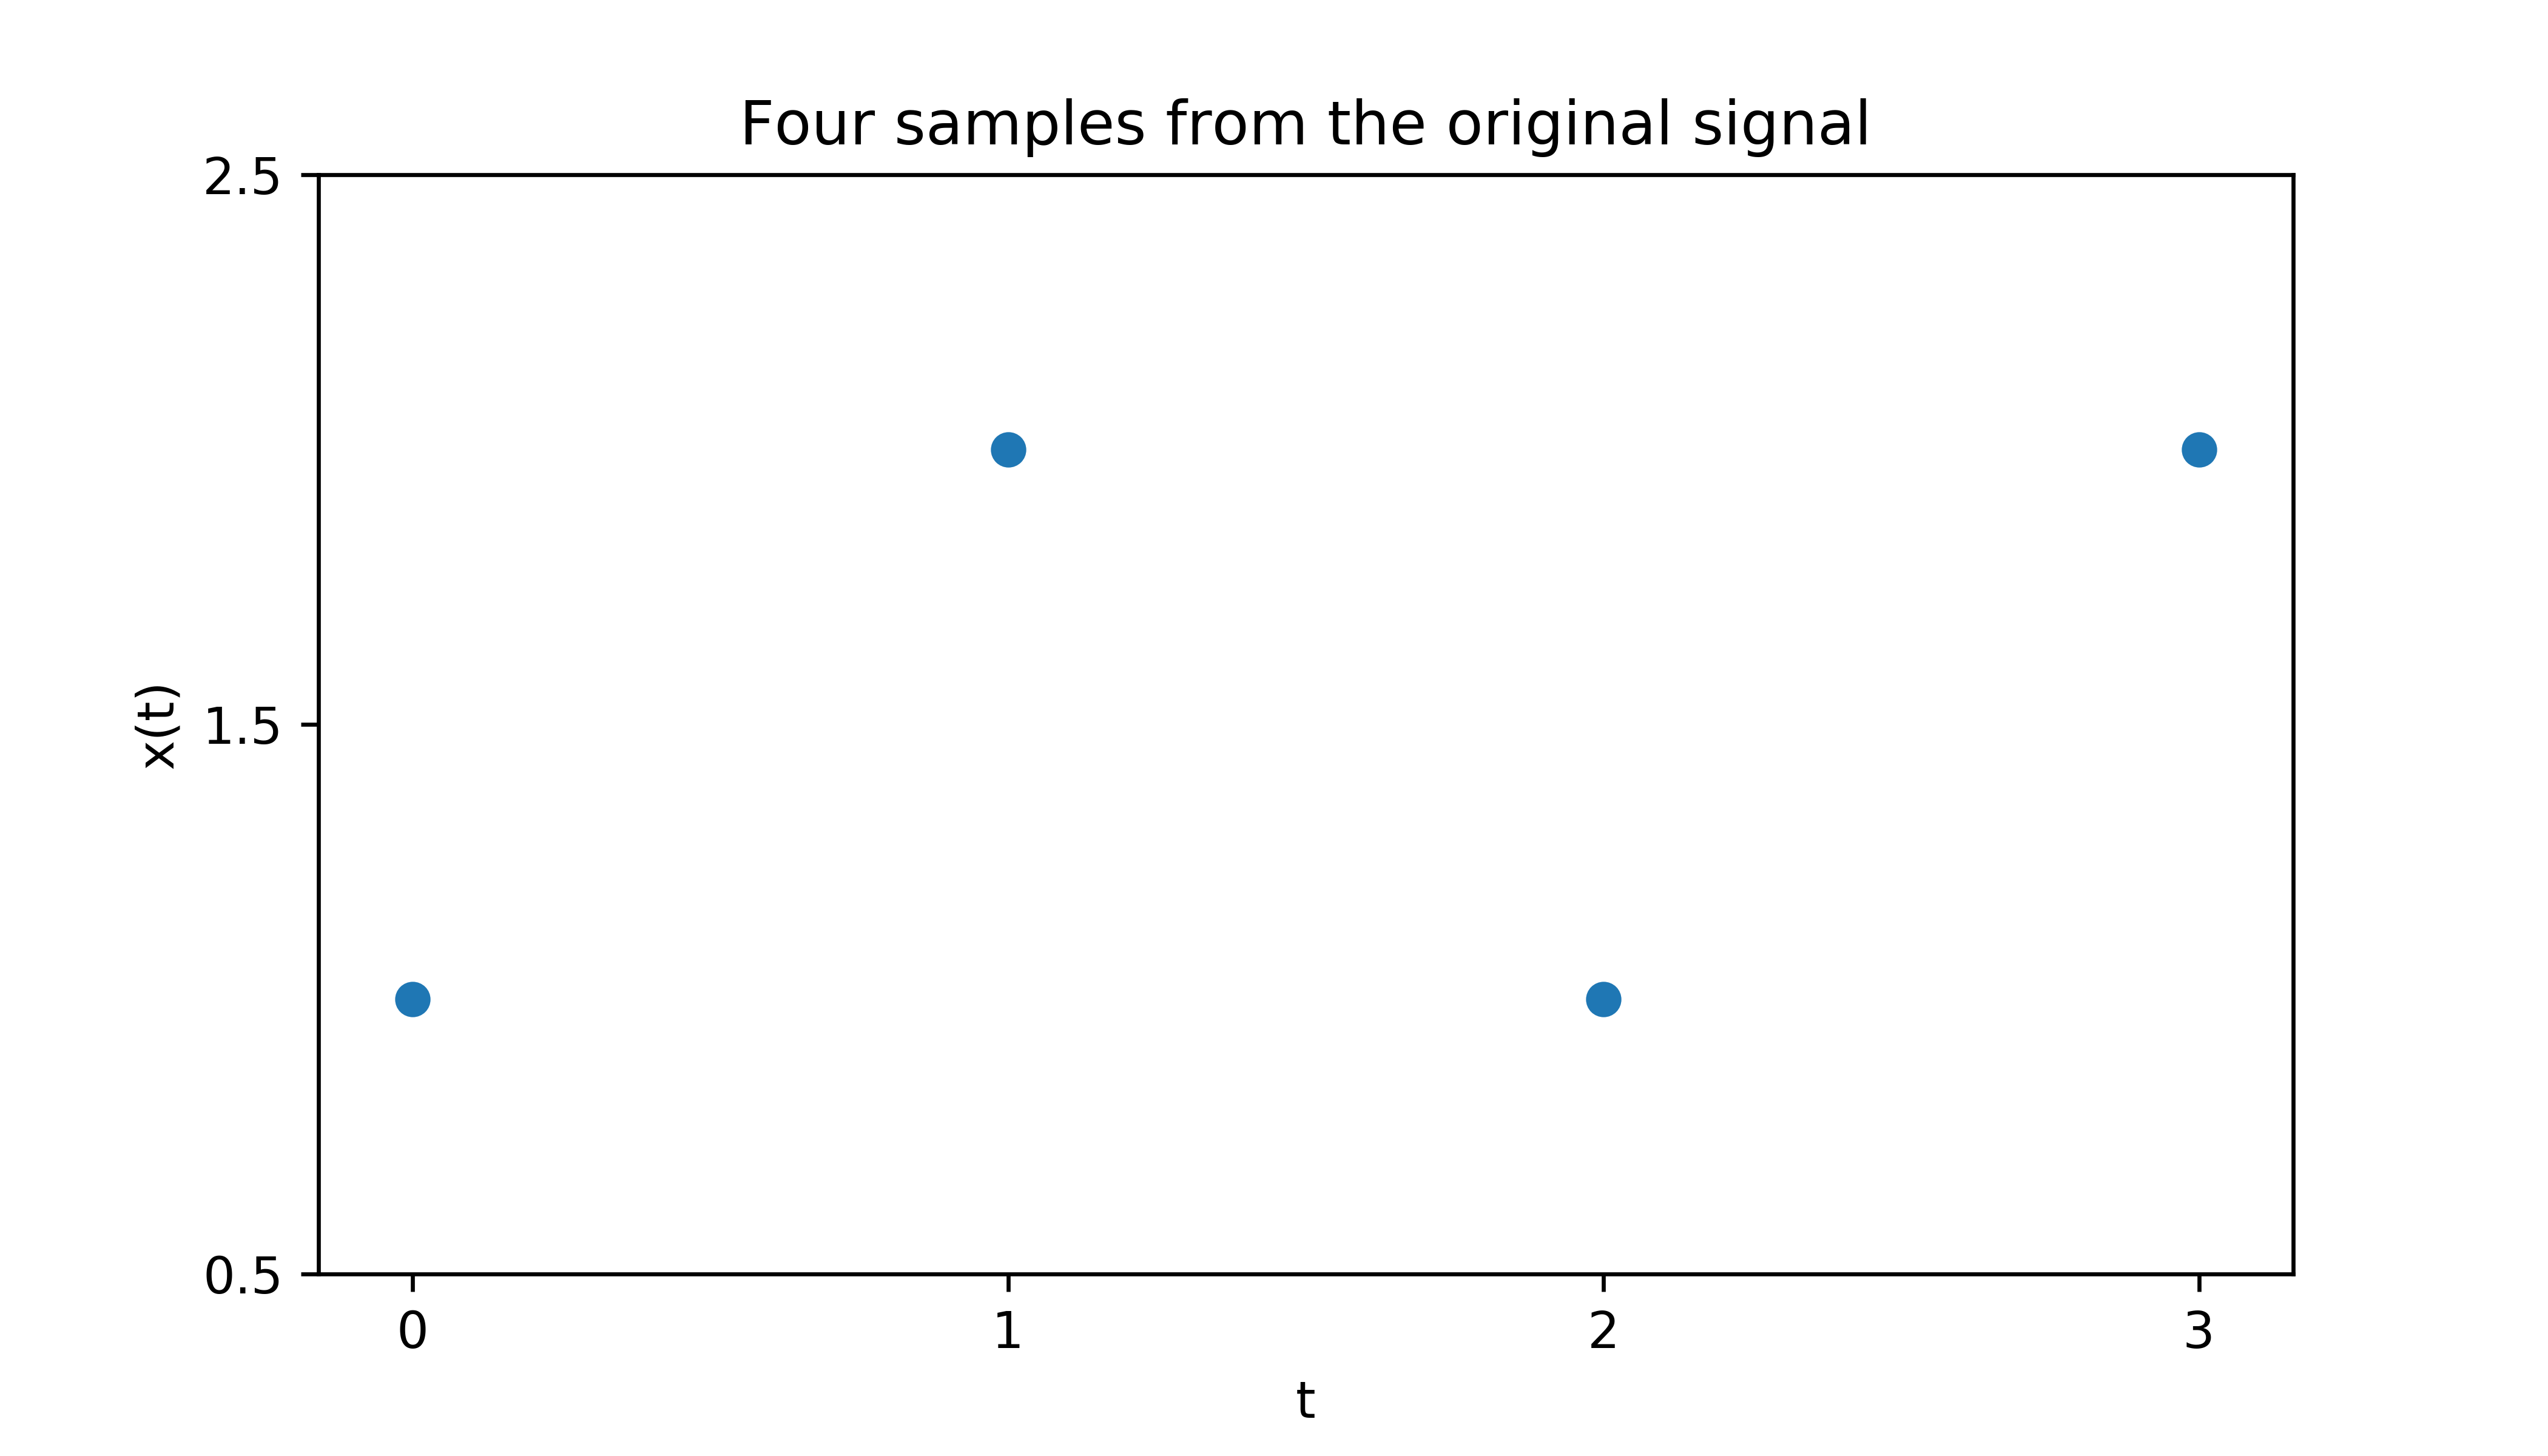
\includegraphics[width=5in]{\bank/interpolation/figures/four_pt_samples}
    \end{center}
  }

  \sol {
    We again resort to the Lagrange Interpolation formula and can arrive at:
    $$x(t) = \frac{(t - 1)(t - 2)(t - 3)}{(-1)(-2)(-3)} + \frac{(t)(t - 2)(t - 3)}{(1)(-1)(-2)} + \frac{(t)(t - 1)(t - 3)}{(2)(1)(-1)} + \frac{(t)(t - 1)(t - 2)}{(3)(2)(1)} = \frac{2}{3} t^3 - 3t^2 + \frac{10}{3} t + 1.$$
    \begin{center}
      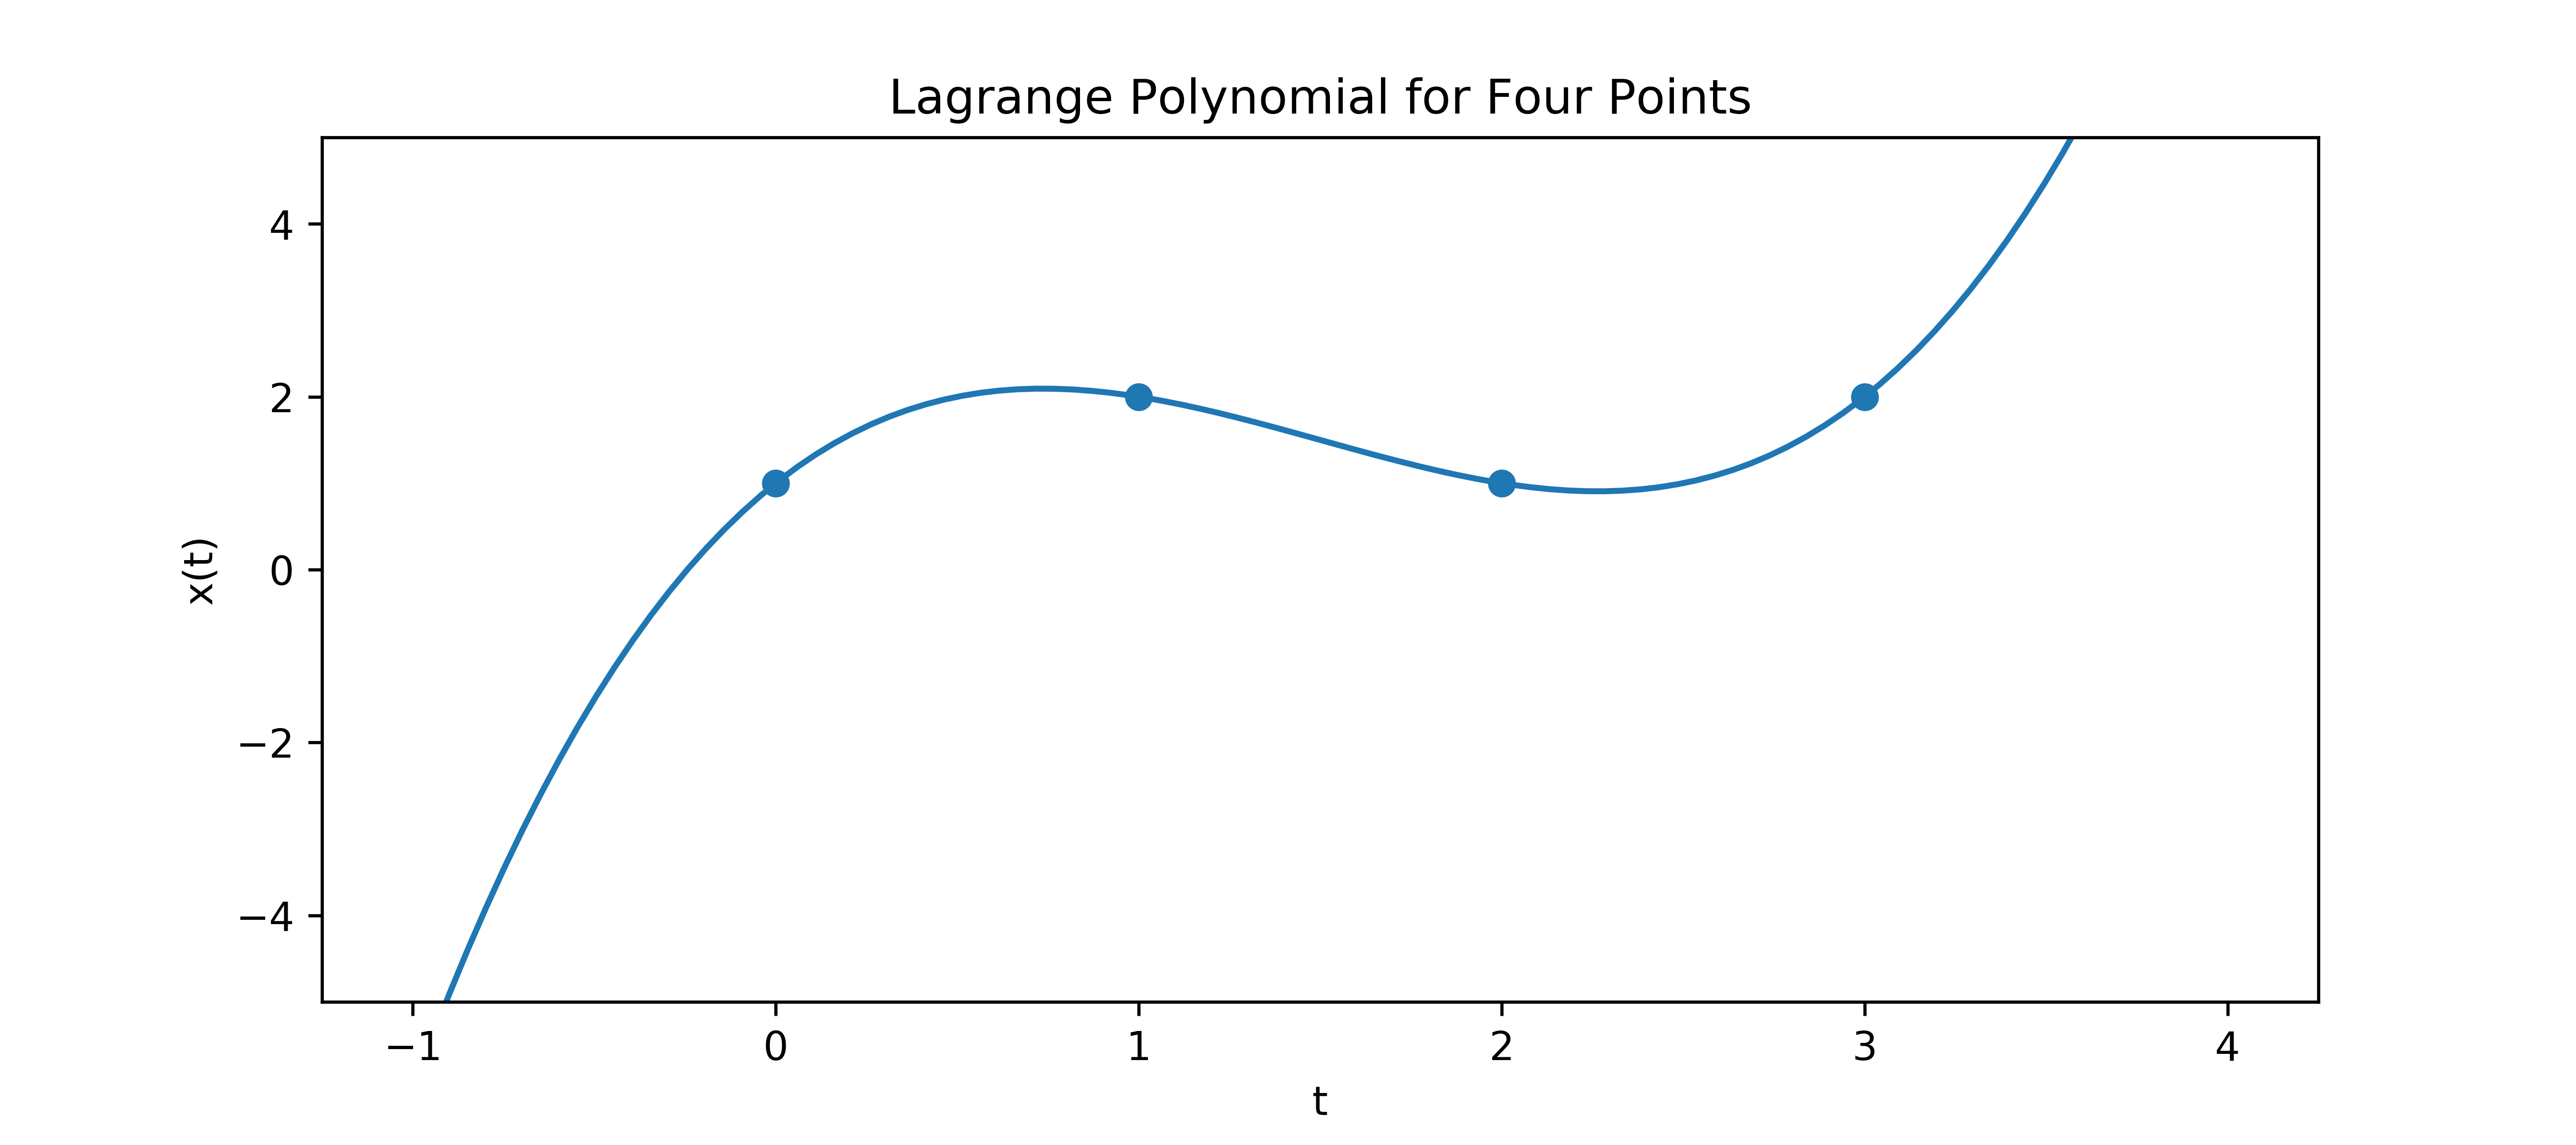
\includegraphics[width=6in]{\bank/interpolation/figures/four_pt_lagrange}
    \end{center}
  }

  \qitem Now let's consider the case in which we take ten samples. First sketch out the interpolated Lagrange Polynomial.
  As we take more samples, what do you notice about the Lagrange polynomials? Are there any concerns we should be making?

  \ws {
    \begin{center}
      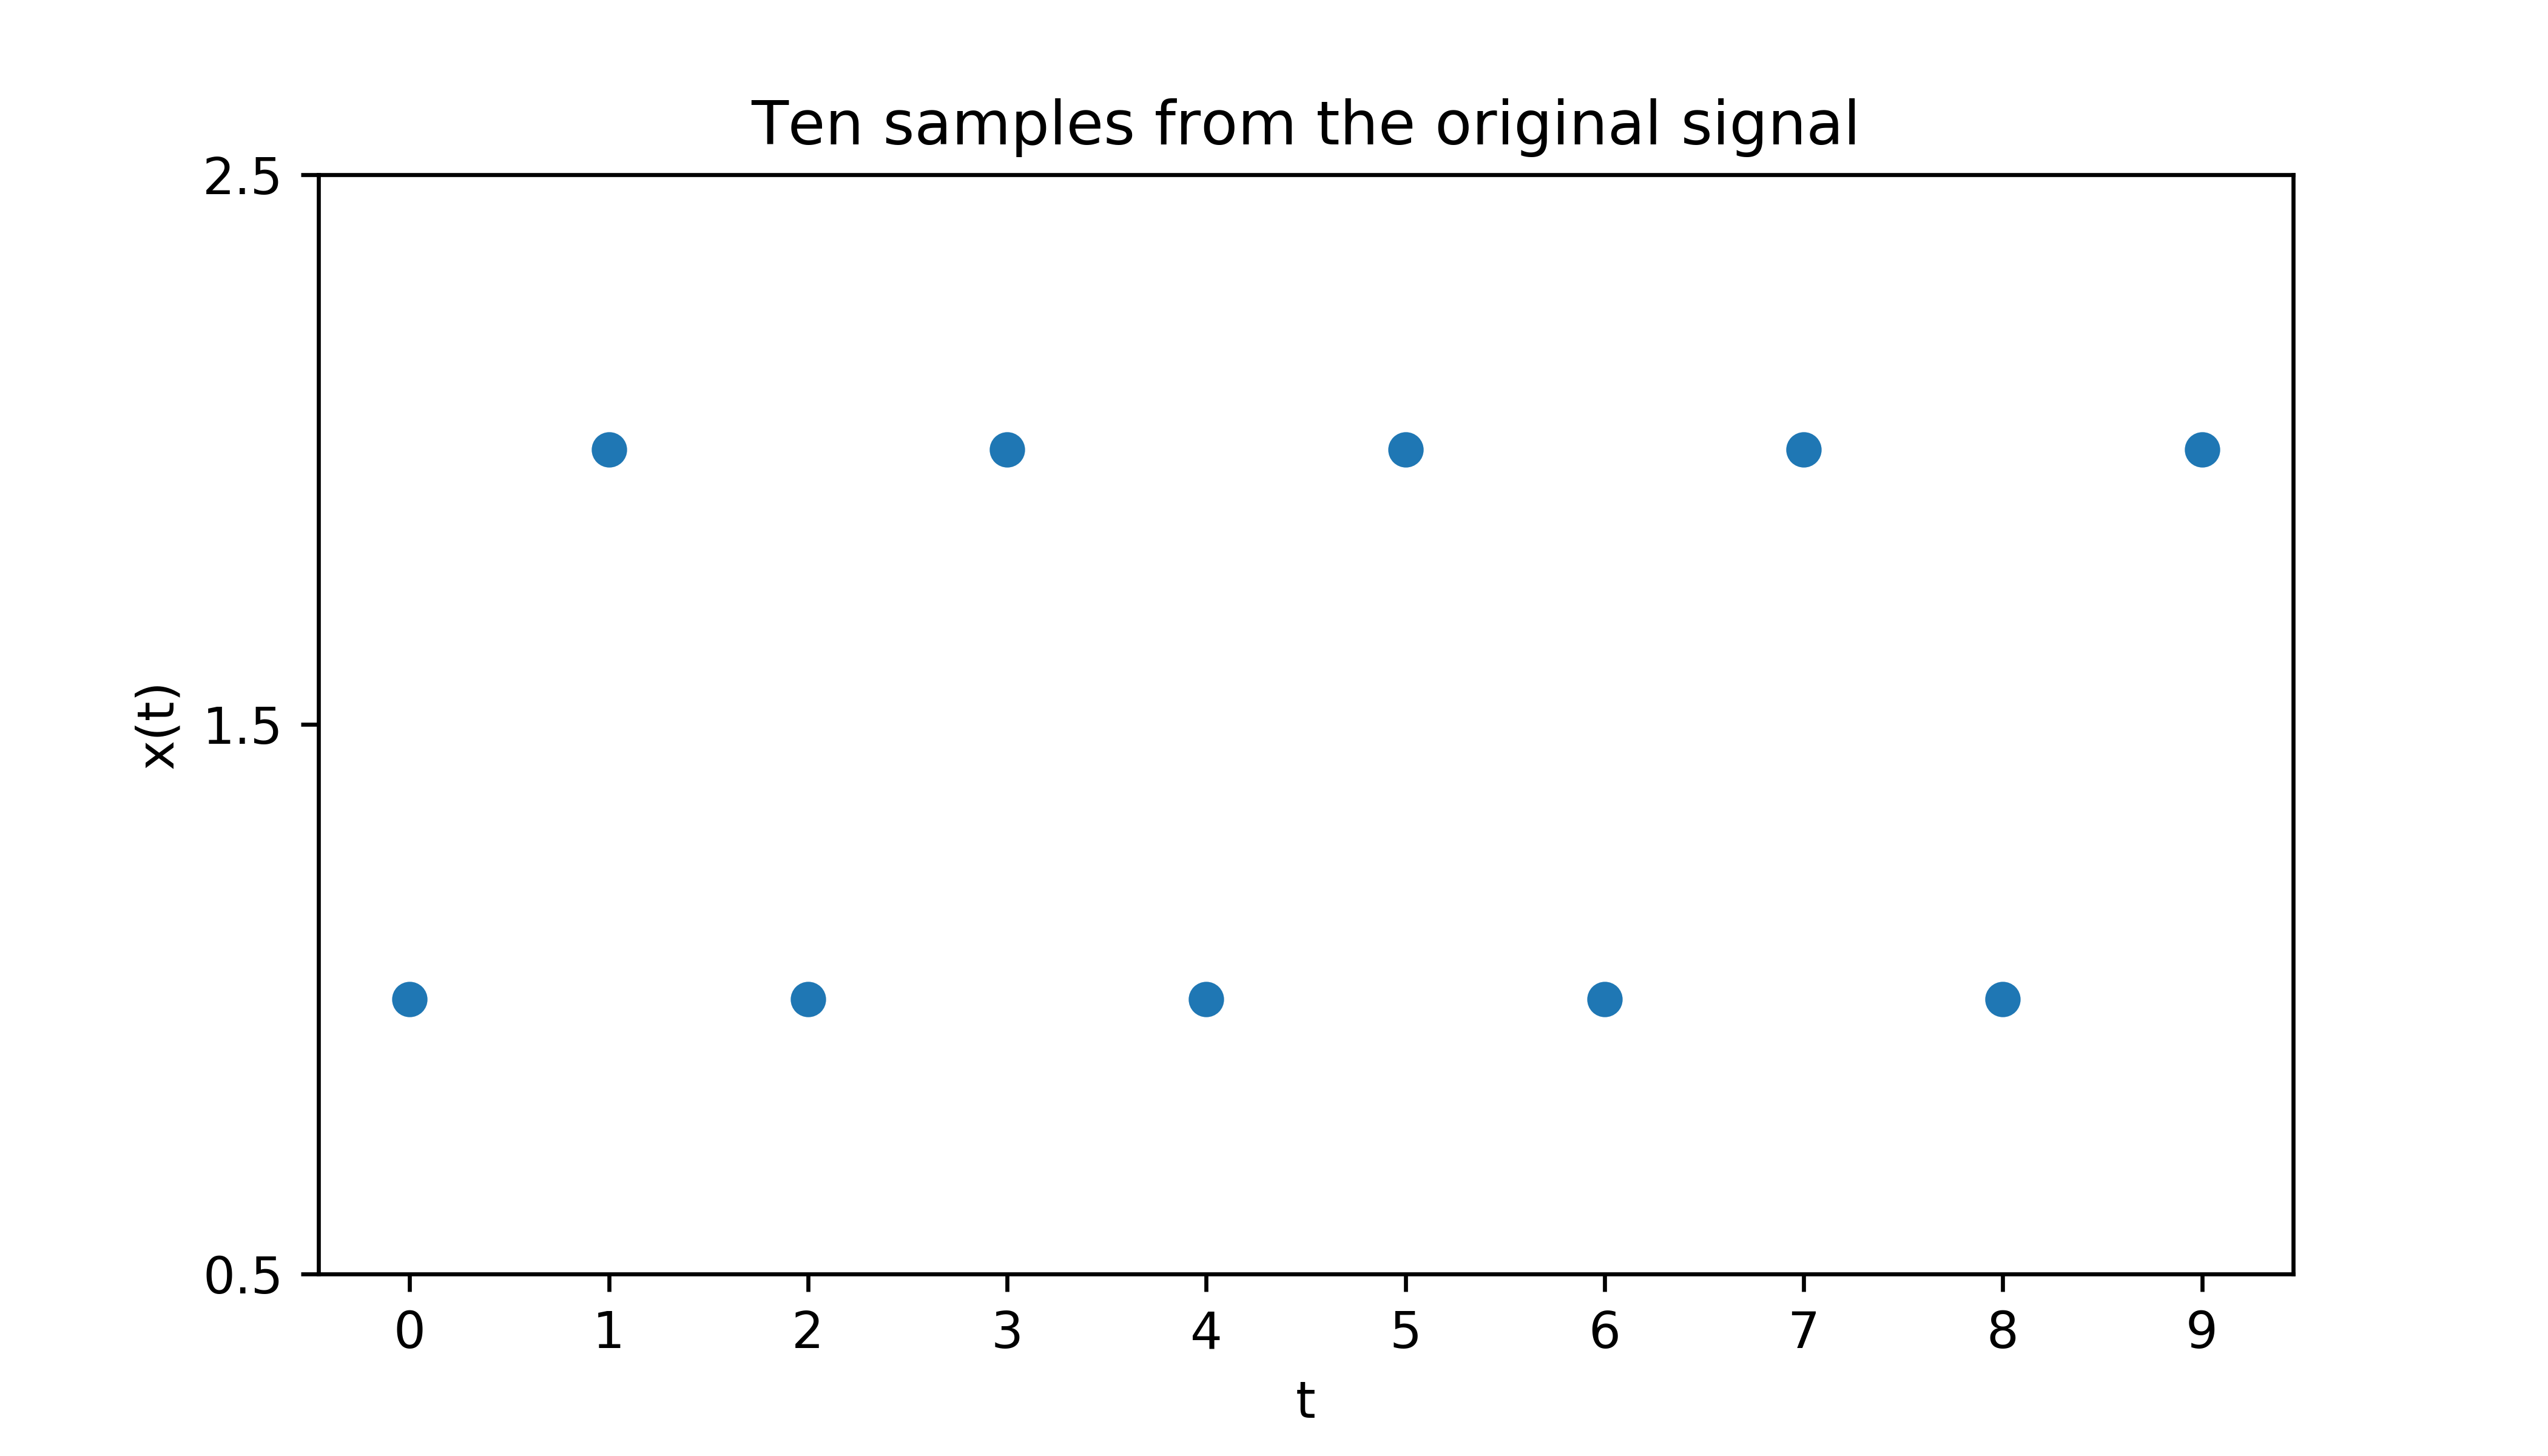
\includegraphics[width=5in]{\bank/interpolation/figures/ten_pt_samples}
    \end{center}
  }

  \sol {
    We will show the result of performing Lagrange Interpolation on these ten samples.
    \begin{center}
      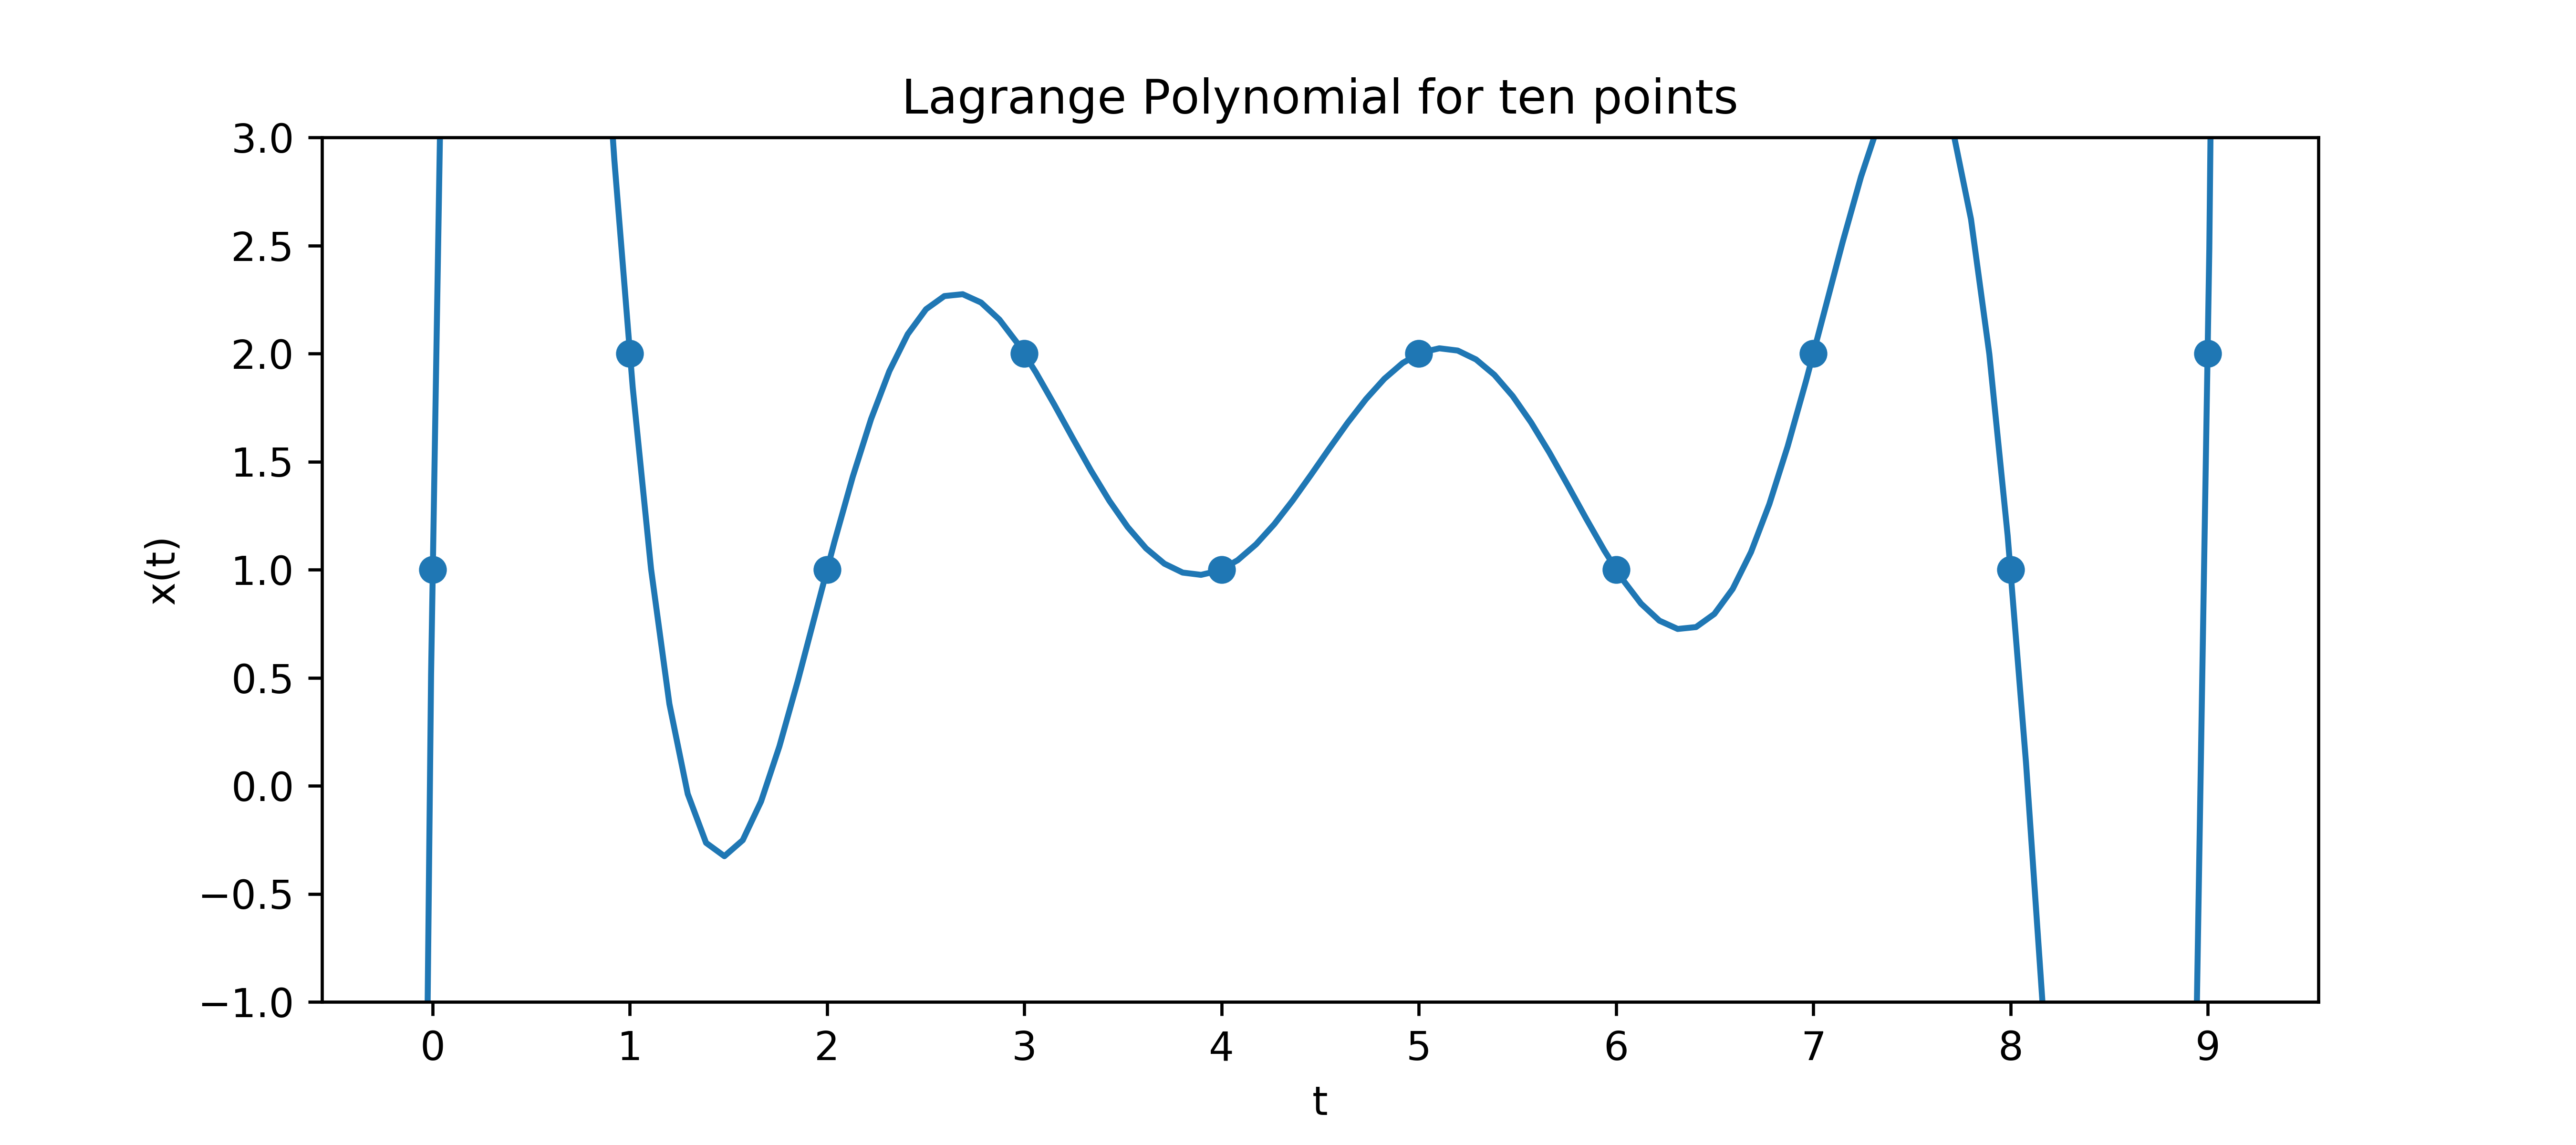
\includegraphics[width=6in]{\bank/interpolation/figures/ten_pt_lagrange}
    \end{center}
    Since Lagrange Interpolation has the constraint that the polynomial must pass through the sampled points, it will perform as expected with the middle points, but as we reach either end, due to the \textbf{polynomial} nature of Lagrange, the interpolation starts becoming unstable. Note that for ten samples, Lagrange will fit a degree nine polynomial, meaning the $t^{9}$ term will drastically increase in magnitude even with small changes in $t.$ 
    In addition, note that both ends of Lagrange Interpolation will diverge to infinity, due to this polynomial nature. Moreso, the left and right ends will alternate between positive and negative infinity, depending on whether the degree of the polynomial is even or odd.
  }

\end{enumerate}

